\begin{frame}
	\myheading{Module 21.2: Intuition behind Variational Autoencoders}
\end{frame}

\begin{frame}
	\begin{columns}
		\column{0.4\textwidth}
		\begin{overlayarea}{\textwidth}{\textheight}
			% LHS: abstraction and generation
			\only<4->{\begin{figure}
				\centering
				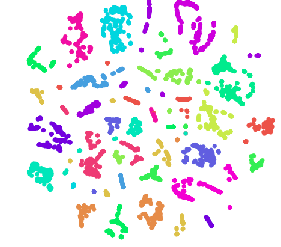
\includegraphics[scale=0.3]{images/abstraction.png}
				\caption{Abstraction}
			\end{figure}}
			\only<5->{\begin{figure}
				\centering
				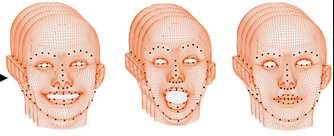
\includegraphics[scale=0.3]{images/faces.png}
				\caption{Generation}
			\end{figure}}
		\end{overlayarea}
		\column{0.6\textwidth}
		\begin{overlayarea}{\textwidth}{\textheight}
			\begin{itemize}\justifying
				\item<1-> Let $\{X = x_i\}_{i=1}^{N}$ be the training data
				\item<2-> We can think of $X$ as a random variable in $R^{n}$
				\item<3-> For example, $X$ could be an image and the dimensions of $X$ correspond to pixels of the image
				\item<4-> We are interested in learning an abstraction (i.e., given an $X$ find the hidden representation $z$)
				\item<5-> We are also interested in generation (i.e., given a hidden representation generate an $X$)
				\item<6-> In probabilistic terms we are interested in $P(z|X)$ and $P(X|z)$  
			\end{itemize}
		\end{overlayarea}
	\end{columns}
\end{frame}


\begin{frame}
	\begin{columns}
		\column{0.4\textwidth}
		\begin{overlayarea}{\textwidth}{\textheight}
			% LHS: show diagram of RBM
			\centering
\vspace{0.5cm}
\tikzstyle{neuronv}=[circle,minimum size=20pt,inner sep=0pt, thick, fill=orange!30, draw=red!50]
\tikzstyle{neuronh}=[circle,minimum size=20pt,inner sep=0pt, thick, fill=blue!20, draw=blue!60]
\tikzstyle{stateTransition}=[thick]
\tikzstyle{learned}=[text=black]
\begin{tikzpicture}[scale=1.9]
    % \draw ;
    \draw[rounded corners=0.5cm, draw=red!60, thick] (-0.4, -0.25) rectangle (2.5, 0.25) {};
    \draw[rounded corners=0.5cm, draw=red!60, thick] (-0.4, 1.25) rectangle (2.5, 1.75) {};

    \node (v1)[neuronv] at (0, 0) {$v_1$};
    \node (v2)[neuronv] at (0.7, 0) {$v_2$};
    \node (v3)[] at (1.4, 0) {$\cdots$};
    \node (v4)[neuronv] at (2.1, 0) {$v_m$};
    \node[below=0.5cm of v2] (v) {$V \in \{0, 1\}^m$};
    \node[learned,below=0.1cm of v1] (bv1) {$b_1$};
    \node[learned,below=0.1cm of v2] (bv2) {$b_2$};
    % \node[learned,below=0.1cm of v3, scale=0.7] (bv3) {$b_{v_3}$};
    \node[learned,below=0.1cm of v4] (bv4) {$b_m$};

    \node (h1)[neuronh] at (0, 1.5) {$h_1$};
    \node (h2)[neuronh] at (0.7, 1.5) {$h_2$};
    \node (h3)[] at (1.4, 1.5) {$\cdots$};
    \node (h4)[neuronh] at (2.1, 1.5) {$h_n$};
    \node[above=0.5cm of h2] (h) {$H \in \{0, 1\}^n$};
    \node[learned,above=0.1cm of h1] (bv1) {$c_1$};
    \node[learned,above=0.1cm of h2] (bv2) {$c_2$};
    % \node[learned,below=0.1cm of v3, scale=0.7] (bv3) {$b_{v_3}$};
    \node[learned,above=0.1cm of h4] (bv4) {$c_n$};

    \node[learned, scale=0.7] (W) at (2.5, 0.75) {$W \in \mathbb{R}^{m \times n}$};

    \draw[learned,stateTransition] (0,0.17) -- (0,1.33) node [midway,left=-0.1cm] {$w_{1,1}$};
    \draw[stateTransition] (0,0.17) -- (0.7,1.33) node [midway,above=-0.06cm,sloped] {};
    \draw[stateTransition] (0,0.17) -- (2.1,1.33) node [midway,above=-0.06cm,sloped] {};

    \draw[stateTransition] (0.7,0.17) -- (0,1.33) node [midway,above=-0.06cm,sloped] {};
    \draw[stateTransition] (0.7,0.17) -- (0.7,1.33) node [midway,above=-0.06cm,sloped] {};
    \draw[stateTransition] (0.7,0.17) -- (2.1,1.33) node [midway,above=-0.06cm,sloped] {};

    \draw[stateTransition] (2.1,0.17) -- (0,1.33) node [midway,above=-0.06cm,sloped] {};
    \draw[stateTransition] (2.1,0.17) -- (0.7,1.33) node [midway,above=-0.06cm,sloped] {};
    \draw[learned,stateTransition] (2.1,0.17) -- (2.1,1.33) node [midway,left=-0.1cm] {$w_{m,n}$};

\end{tikzpicture}			
		\end{overlayarea}
		\column{0.6\textwidth}
		\begin{overlayarea}{\textwidth}{\textheight}
			\begin{itemize}\justifying
				\item<1-> Earlier we saw RBMs where we learnt $P(z|X)$ and $P(X|z)$ (to be consistent with the literation on VAEs we will use $z$ instead of $H$ and $X$ instead of $V$) 
				\item<2-> Below we list certain characteristics of RBMs
				\item<3-> \textbf{Structural assumptions:} We assumed certain independencies in the Markov Network
				\item<4-> \textbf{Computational:} When training with Gibbs Sampling we have to run the Markov Chain for many time steps which is expensive 
				\item<5-> \textbf{Approximation:} When using Contrastive Divergence, we approximate the expectation by a point estimate
				% \item<6-> (Nothing wrong with the above but we just mention them to make the reader aware of these characteristics)
			\end{itemize}
		\end{overlayarea}
	\end{columns}
\end{frame}


\begin{frame}
	\begin{columns}
		\column{0.4\textwidth}
		\begin{overlayarea}{\textwidth}{\textheight}
			% \centering
\vspace{0.5cm}
\tikzstyle{neuronv}=[circle,minimum size=20pt,inner sep=0pt, thick, fill=orange!30, draw=red!50]
\tikzstyle{neuronh}=[circle,minimum size=20pt,inner sep=0pt, thick, fill=blue!20, draw=blue!60]
\tikzstyle{stateTransition}=[thick]
\tikzstyle{learned}=[text=black]
\begin{tikzpicture}[scale=1.9]
    % \draw ;
    \draw[rounded corners=0.5cm, draw=red!60, thick] (-0.4, -0.25) rectangle (2.5, 0.25) {};
    \draw[rounded corners=0.5cm, draw=red!60, thick] (-0.4, 1.25) rectangle (2.5, 1.75) {};

    \node (v1)[neuronv] at (0, 0) {$v_1$};
    \node (v2)[neuronv] at (0.7, 0) {$v_2$};
    \node (v3)[] at (1.4, 0) {$\cdots$};
    \node (v4)[neuronv] at (2.1, 0) {$v_m$};
    \node[below=0.5cm of v2] (v) {$V \in \{0, 1\}^m$};
    \node[learned,below=0.1cm of v1] (bv1) {$b_1$};
    \node[learned,below=0.1cm of v2] (bv2) {$b_2$};
    % \node[learned,below=0.1cm of v3, scale=0.7] (bv3) {$b_{v_3}$};
    \node[learned,below=0.1cm of v4] (bv4) {$b_m$};

    \node (h1)[neuronh] at (0, 1.5) {$h_1$};
    \node (h2)[neuronh] at (0.7, 1.5) {$h_2$};
    \node (h3)[] at (1.4, 1.5) {$\cdots$};
    \node (h4)[neuronh] at (2.1, 1.5) {$h_n$};
    \node[above=0.5cm of h2] (h) {$H \in \{0, 1\}^n$};
    \node[learned,above=0.1cm of h1] (bv1) {$c_1$};
    \node[learned,above=0.1cm of h2] (bv2) {$c_2$};
    % \node[learned,below=0.1cm of v3, scale=0.7] (bv3) {$b_{v_3}$};
    \node[learned,above=0.1cm of h4] (bv4) {$c_n$};

    \node[learned, scale=0.7] (W) at (2.5, 0.75) {$W \in \mathbb{R}^{m \times n}$};

    \draw[learned,stateTransition] (0,0.17) -- (0,1.33) node [midway,left=-0.1cm] {$w_{1,1}$};
    \draw[stateTransition] (0,0.17) -- (0.7,1.33) node [midway,above=-0.06cm,sloped] {};
    \draw[stateTransition] (0,0.17) -- (2.1,1.33) node [midway,above=-0.06cm,sloped] {};

    \draw[stateTransition] (0.7,0.17) -- (0,1.33) node [midway,above=-0.06cm,sloped] {};
    \draw[stateTransition] (0.7,0.17) -- (0.7,1.33) node [midway,above=-0.06cm,sloped] {};
    \draw[stateTransition] (0.7,0.17) -- (2.1,1.33) node [midway,above=-0.06cm,sloped] {};

    \draw[stateTransition] (2.1,0.17) -- (0,1.33) node [midway,above=-0.06cm,sloped] {};
    \draw[stateTransition] (2.1,0.17) -- (0.7,1.33) node [midway,above=-0.06cm,sloped] {};
    \draw[learned,stateTransition] (2.1,0.17) -- (2.1,1.33) node [midway,left=-0.1cm] {$w_{m,n}$};

\end{tikzpicture}
			\vspace{3pt}
			\tikzstyle{input_neuron}=[circle,draw=red!50,fill=red!10,thick,minimum size=6mm]
\tikzstyle{hidden_neuron}=[circle,draw=blue!50,fill=cyan!10,thick,minimum size=6mm]
\tikzstyle{output_neuron}=[circle,draw=green!50,fill=green!10,thick,minimum size=6mm]

\tikzstyle{input}=[circle,draw=black!50,fill=black!20,thick,minimum size=6mm]

\begin{center}
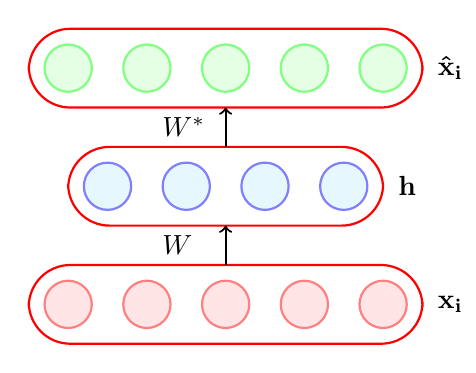
\begin{tikzpicture}

\node [input_neuron] (neuron01) at (6.5,4.5) {};
\node [input_neuron] (neuron02) at (7.5,4.5){};
\node [input_neuron] (neuron03) at (8.5,4.5) {};
\node [input_neuron] (neuron04) at (9.5,4.5) {};
\node [input_neuron] (neuron05) at (10.5,4.5) {};
\node [hidden_neuron] (neuron51) at (7,6) {} ;
\node [hidden_neuron] (neuron52) at (8,6)  {};
\node [hidden_neuron] (neuron53) at (9,6)  {};
\node [hidden_neuron] (neuron54) at (10,6)  {};

\node [output_neuron] (neuron11) at (6.5,7.5)  {};
\node [output_neuron] (neuron12) at (7.5,7.5)  {};
\node [output_neuron] (neuron13) at (8.5,7.5)  {};
\node [output_neuron] (neuron14) at (9.5,7.5)  {};
\node [output_neuron] (neuron15) at (10.5,7.5)  {};

\node[text width=0.01cm] at (11.2,4.5) {$\mathbf{x_i}$};
\node[text width=0.007cm] at (7.7,5.25) {$W$};
\node[text width=0.01cm] at (10.7,6) {$\mathbf{h}$};
\node[text width=0.007cm] at (7.7,6.75) {$W^*$};
\node[text width=0.01cm] at (11.2,7.5) {$\mathbf{\hat{x}_i}$};

\draw[red!100,thick,solid,rounded corners=15pt] (6,4) rectangle (11,5);
\draw[red!100,thick,solid,rounded corners=15pt] (6.5,5.5) rectangle (10.5,6.5);
\draw[red!100,thick,solid,rounded corners=15pt] (6,7) rectangle (11,8);



\draw[thick,->] (8.5,5) -- (8.5,5.5);

\draw[thick,->] (8.5,6.5) -- (8.5,7);



\end{tikzpicture}
\end{center}

		\end{overlayarea}
		\column{0.6\textwidth}
		\begin{overlayarea}{\textwidth}{\textheight}
			\begin{itemize}\justifying
				\item<1-> We will now look at Variational Autoencoders which also learn $P(z|X)$ and $P(X|z)$ but using a very different approach
				\item<2-> Recall that in RBMS we learned the parameters by solving the following optimization problem
				\begin{align*}
					maximize \prod_{i=1}^{N} P(X = x_i)
				\end{align*}
				\item<3-> In VAEs also we will start with the same objective function but use a different trick to solve the optimization problem (we will get there soon)
			\end{itemize}
		\end{overlayarea}
	\end{columns}
\end{frame}


\begin{frame}
	\begin{columns}
		\column{0.4\textwidth}
		\begin{overlayarea}{\textwidth}{\textheight}
			\vspace{3pt}
			\tikzstyle{input_neuron}=[circle,draw=red!50,fill=red!10,thick,minimum size=6mm]
\tikzstyle{hidden_neuron}=[circle,draw=blue!50,fill=cyan!10,thick,minimum size=6mm]
\tikzstyle{output_neuron}=[circle,draw=green!50,fill=green!10,thick,minimum size=6mm]

\tikzstyle{input}=[circle,draw=black!50,fill=black!20,thick,minimum size=6mm]

\begin{center}
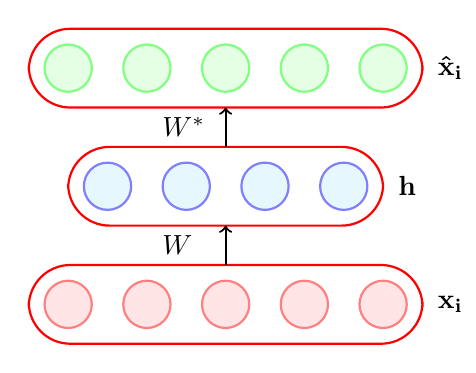
\begin{tikzpicture}

\node [input_neuron] (neuron01) at (6.5,4.5) {};
\node [input_neuron] (neuron02) at (7.5,4.5){};
\node [input_neuron] (neuron03) at (8.5,4.5) {};
\node [input_neuron] (neuron04) at (9.5,4.5) {};
\node [input_neuron] (neuron05) at (10.5,4.5) {};
\node [hidden_neuron] (neuron51) at (7,6) {} ;
\node [hidden_neuron] (neuron52) at (8,6)  {};
\node [hidden_neuron] (neuron53) at (9,6)  {};
\node [hidden_neuron] (neuron54) at (10,6)  {};

\node [output_neuron] (neuron11) at (6.5,7.5)  {};
\node [output_neuron] (neuron12) at (7.5,7.5)  {};
\node [output_neuron] (neuron13) at (8.5,7.5)  {};
\node [output_neuron] (neuron14) at (9.5,7.5)  {};
\node [output_neuron] (neuron15) at (10.5,7.5)  {};

\node[text width=0.01cm] at (11.2,4.5) {$\mathbf{x_i}$};
\node[text width=0.007cm] at (7.7,5.25) {$W$};
\node[text width=0.01cm] at (10.7,6) {$\mathbf{h}$};
\node[text width=0.007cm] at (7.7,6.75) {$W^*$};
\node[text width=0.01cm] at (11.2,7.5) {$\mathbf{\hat{x}_i}$};

\draw[red!100,thick,solid,rounded corners=15pt] (6,4) rectangle (11,5);
\draw[red!100,thick,solid,rounded corners=15pt] (6.5,5.5) rectangle (10.5,6.5);
\draw[red!100,thick,solid,rounded corners=15pt] (6,7) rectangle (11,8);



\draw[thick,->] (8.5,5) -- (8.5,5.5);

\draw[thick,->] (8.5,6.5) -- (8.5,7);



\end{tikzpicture}
\end{center}

		\end{overlayarea}
		\column{0.6\textwidth}
		\begin{overlayarea}{\textwidth}{\textheight}
			\begin{itemize}\justifying
				\item<1-> Goal 1: Learn a distribution over the latent variables ($P(z|X)$)
				\item<2-> Goal 2: Learn a distribution over the visible variables ($P(X|z)$)
				\item<3-> Suppose we assume a certain form for the distribution $P(z|X)$ 
				\item<4-> For example, let us assume that $P(z|X)$ is a Normal distribution 
				\item<5-> In RBMs, we had assumed a certain structure (independencies) for the joint distribution whereas here we are assuming a certain family form for the distribution $P(z|X)$ 
			\end{itemize}
		\end{overlayarea}
	\end{columns}
\end{frame}


\begin{frame}
	\begin{columns}
		\column{0.4\textwidth}
		\begin{overlayarea}{\textwidth}{\textheight}
			\vspace{3pt}
			\tikzstyle{input_neuron}=[circle,draw=red!50,fill=red!10,thick,minimum size=6mm]
\tikzstyle{hidden_neuron}=[circle,draw=blue!50,fill=cyan!10,thick,minimum size=6mm]
\tikzstyle{output_neuron}=[circle,draw=green!50,fill=green!10,thick,minimum size=6mm]

\tikzstyle{input}=[circle,draw=black!50,fill=black!20,thick,minimum size=6mm]

\begin{center}
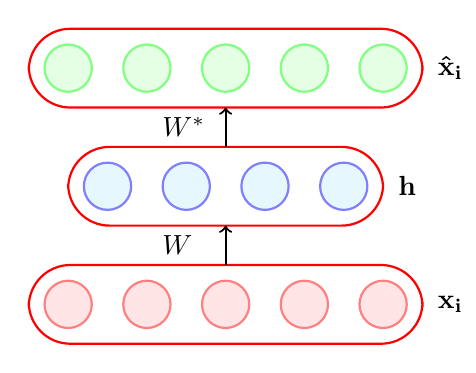
\begin{tikzpicture}

\node [input_neuron] (neuron01) at (6.5,4.5) {};
\node [input_neuron] (neuron02) at (7.5,4.5){};
\node [input_neuron] (neuron03) at (8.5,4.5) {};
\node [input_neuron] (neuron04) at (9.5,4.5) {};
\node [input_neuron] (neuron05) at (10.5,4.5) {};
\node [hidden_neuron] (neuron51) at (7,6) {} ;
\node [hidden_neuron] (neuron52) at (8,6)  {};
\node [hidden_neuron] (neuron53) at (9,6)  {};
\node [hidden_neuron] (neuron54) at (10,6)  {};

\node [output_neuron] (neuron11) at (6.5,7.5)  {};
\node [output_neuron] (neuron12) at (7.5,7.5)  {};
\node [output_neuron] (neuron13) at (8.5,7.5)  {};
\node [output_neuron] (neuron14) at (9.5,7.5)  {};
\node [output_neuron] (neuron15) at (10.5,7.5)  {};

\node[text width=0.01cm] at (11.2,4.5) {$\mathbf{x_i}$};
\node[text width=0.007cm] at (7.7,5.25) {$W$};
\node[text width=0.01cm] at (10.7,6) {$\mathbf{h}$};
\node[text width=0.007cm] at (7.7,6.75) {$W^*$};
\node[text width=0.01cm] at (11.2,7.5) {$\mathbf{\hat{x}_i}$};

\draw[red!100,thick,solid,rounded corners=15pt] (6,4) rectangle (11,5);
\draw[red!100,thick,solid,rounded corners=15pt] (6.5,5.5) rectangle (10.5,6.5);
\draw[red!100,thick,solid,rounded corners=15pt] (6,7) rectangle (11,8);



\draw[thick,->] (8.5,5) -- (8.5,5.5);

\draw[thick,->] (8.5,6.5) -- (8.5,7);



\end{tikzpicture}
\end{center}

		\end{overlayarea}
		\column{0.6\textwidth}
		\begin{overlayarea}{\textwidth}{\textheight}
			\begin{itemize}\justifying
				\item<1-> Now given the assumption that $P(z|X)$ is a Normal distribution can you think of adapting the autoencoder architecture to learn the distribution $P(z|X)$ instead of learning $z$
				\item<2-> What do we mean when we say we want to learn a distribution? We mean that we want to learn the parameters of the distribution
				\item<3-> What are the parameters of a Normal Distribution? Mean ($\mu$) and Variance ($\sigma$)
				\item<4-> So now what would you want the embedding generated by the encoder to represent ?
				\item<5-> Well, we could design the encoder to predict the mean and variance of $P(z|X)$
			\end{itemize}
		\end{overlayarea}
	\end{columns}
\end{frame}


\begin{frame}
	\begin{columns}
		\column{0.4\textwidth}
		\begin{overlayarea}{\textwidth}{\textheight}
			\vspace{3pt}
			\tikzstyle{input_neuron}=[circle,draw=red!50,fill=red!10,thick,minimum size=6mm]
\tikzstyle{hidden_neuron}=[circle,draw=blue!50,fill=cyan!10,thick,minimum size=6mm]
\tikzstyle{output_neuron}=[circle,draw=green!50,fill=green!10,thick,minimum size=6mm]

\tikzstyle{input}=[circle,draw=black!50,fill=black!20,thick,minimum size=6mm]

\begin{center}
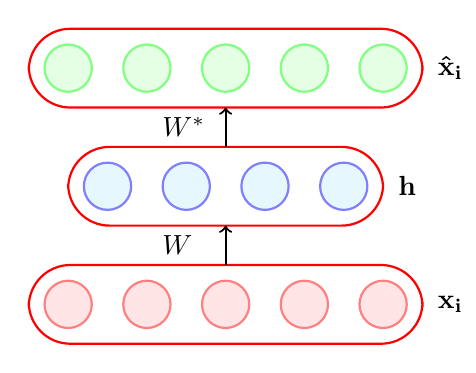
\begin{tikzpicture}

\node [input_neuron] (neuron01) at (6.5,4.5) {};
\node [input_neuron] (neuron02) at (7.5,4.5){};
\node [input_neuron] (neuron03) at (8.5,4.5) {};
\node [input_neuron] (neuron04) at (9.5,4.5) {};
\node [input_neuron] (neuron05) at (10.5,4.5) {};
\node [hidden_neuron] (neuron51) at (7,6) {} ;
\node [hidden_neuron] (neuron52) at (8,6)  {};
\node [hidden_neuron] (neuron53) at (9,6)  {};
\node [hidden_neuron] (neuron54) at (10,6)  {};

\node [output_neuron] (neuron11) at (6.5,7.5)  {};
\node [output_neuron] (neuron12) at (7.5,7.5)  {};
\node [output_neuron] (neuron13) at (8.5,7.5)  {};
\node [output_neuron] (neuron14) at (9.5,7.5)  {};
\node [output_neuron] (neuron15) at (10.5,7.5)  {};

\node[text width=0.01cm] at (11.2,4.5) {$\mathbf{x_i}$};
\node[text width=0.007cm] at (7.7,5.25) {$W$};
\node[text width=0.01cm] at (10.7,6) {$\mathbf{h}$};
\node[text width=0.007cm] at (7.7,6.75) {$W^*$};
\node[text width=0.01cm] at (11.2,7.5) {$\mathbf{\hat{x}_i}$};

\draw[red!100,thick,solid,rounded corners=15pt] (6,4) rectangle (11,5);
\draw[red!100,thick,solid,rounded corners=15pt] (6.5,5.5) rectangle (10.5,6.5);
\draw[red!100,thick,solid,rounded corners=15pt] (6,7) rectangle (11,8);



\draw[thick,->] (8.5,5) -- (8.5,5.5);

\draw[thick,->] (8.5,6.5) -- (8.5,7);



\end{tikzpicture}
\end{center}

		\end{overlayarea}
		\column{0.6\textwidth}
		\begin{overlayarea}{\textwidth}{\textheight}
			\begin{itemize}\justifying
				\item<1-> But how will we train the encoder ?
				\item<2-> What is the loss function that we will use ?
				\item<3-> More specifically, how will we ensure that the $\mu$ and $\sigma$ that the encoder produces are the true $\mu$ and $\sigma$ of $P(z|X)$
				\item<4-> We don't even know what the true $\mu$ and $\sigma$ are then how to we guide/train the model to produce these $\mu$ and $\sigma$
				\item<5-> \textbf{Spoiler Alert:} We will be making some assumptions but to see why these assumptions make sense we will first revisit the concept of latent variables
			\end{itemize}
		\end{overlayarea}
	\end{columns}
\end{frame}


\begin{frame}
	\begin{columns}
		\column{0.4\textwidth}
		\begin{overlayarea}{\textwidth}{\textheight}
			% LHS: show some images of MNIST
			\vspace{3pt}
			\begin{figure}
				\centering
				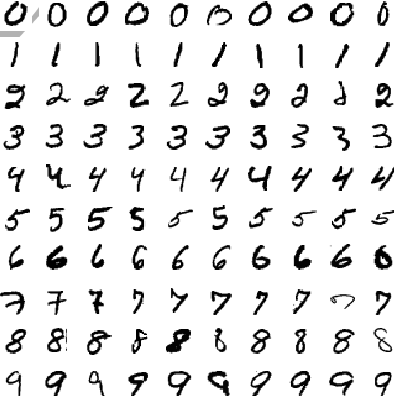
\includegraphics[scale=0.3]{images/mnist.png}
			\end{figure}
		\end{overlayarea}
		\column{0.6\textwidth}
		\begin{overlayarea}{\textwidth}{\textheight}
			\begin{itemize}\justifying
				\item<1-> Consider images of handwritten digits where visible random variables are the pixels of the image
				\item<2-> And we can think of several latent variables ($z$): the digit, size, angle, thickness, position and so on
				\item<3-> It is reasonable to argue that once we select a $z$, the image is actually a deterministic function of $z$
				\item<4-> For example, once the digit, size, angle thickness, position, \textit{etc.} are fixed we know exactly what the image should look like
				\item<5-> Of course, we are assuming that we have enough latent variables to capture all characteristics of handwritten digits 
			\end{itemize}
		\end{overlayarea}
	\end{columns}
\end{frame}


\begin{frame}
	\begin{columns}
		\column{0.4\textwidth}
		\begin{overlayarea}{\textwidth}{\textheight}
			\vspace{3pt}
			\begin{figure}
				\centering
				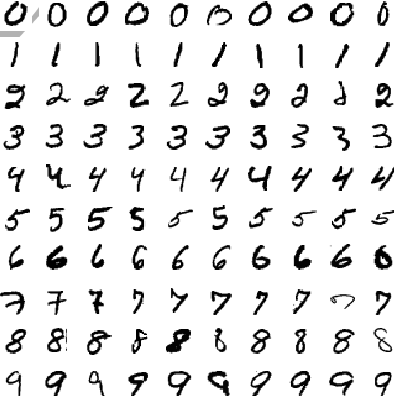
\includegraphics[scale=0.3]{images/mnist.png}
			\end{figure}
		\end{overlayarea}
		\column{0.6\textwidth}
		\begin{overlayarea}{\textwidth}{\textheight}
			\begin{itemize}\justifying
				\item<1-> Of course, even though deterministic, the image (or visible variables) may still be a complex function of the hidden variables $z$
				\item<2-> In others words, $X = f (z; \theta)$ where $z$ is a complex function and $\theta$ are the parameters of this complex function
				\item<3-> Can you think of how you could model such a complex function ? 
				\item<4-> Well, we could use a deep neural network which is good at approximating arbitrary complex functions (recall Universal Approximation Theorem)
				\item<5-> With this intuition, we will now look at the full picture and discuss the objective function
			\end{itemize}
		\end{overlayarea}
	\end{columns}
\end{frame}


\begin{frame}
	\begin{columns}
		\column{0.4\textwidth}
		\begin{overlayarea}{\textwidth}{\textheight}
			% LHS: Show the VAE diagram the VAE tutorial but one step at a time synced with the bullets
			\vspace{4mm}
			\begin{tikzpicture}
				\node[inner sep=0pt] (encoder) at (0,0) {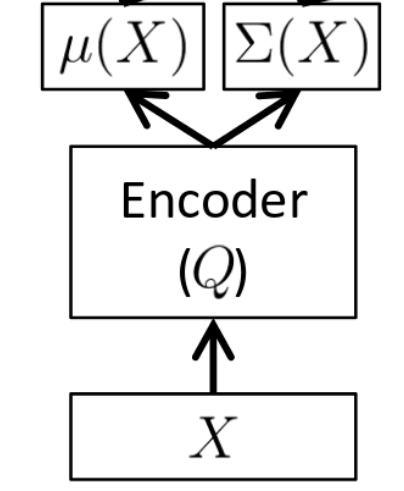
\includegraphics[scale=0.15]{images/vae_encoder.png}};
				\onslide<3->{\node[inner sep=0pt] (sample) at (0,2) {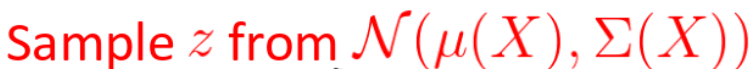
\includegraphics[scale=0.15]{images/vae_sample.png}};
				\draw[->,thick] (encoder.north) -- (sample.south);
				}
				\onslide<4->{\node[inner sep=0pt] (decoder) at (0,4) {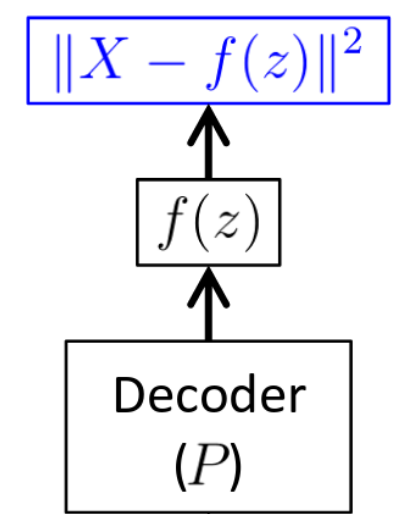
\includegraphics[scale=0.15]{images/vae_decoder.png}};
				\draw[->,thick] (sample.north) -- (decoder.south);
				}
			\end{tikzpicture}
		\end{overlayarea}
		\column{0.6\textwidth}
		\begin{overlayarea}{\textwidth}{\textheight}
			\begin{itemize}\justifying
				\item<1-> First, the task of the encoder is to predict the parameters $(\mu, \sigma)$ of $P(z|X)$
				\item<2-> So given a training sample $X$, the encoder will first produce $\mu(X), \sigma(X)$
				\item<3-> We will now sample a hidden variable $z$ from the distribution $N(\mu(X), \sigma(X))$
				\item<4-> The job of the decoder is to then reconstruct X from this sampled $z$
			\end{itemize}
		\end{overlayarea}
	\end{columns}
\end{frame}


\begin{frame}
	\begin{columns}
		\column{0.4\textwidth}
		\begin{overlayarea}{\textwidth}{\textheight}
			\vspace{4mm}
			\begin{tikzpicture}
				\node[inner sep=0pt] (encoder) at (0,0) {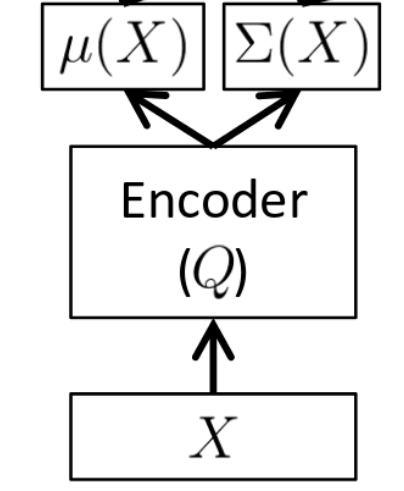
\includegraphics[scale=0.15]{images/vae_encoder.png}};
				\node[inner sep=0pt] (sample) at (0,2) {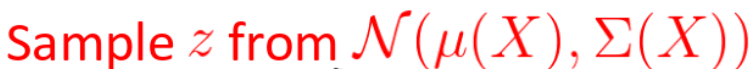
\includegraphics[scale=0.15]{images/vae_sample.png}};
				\draw[->,thick] (encoder.north) -- (sample.south);
				\node[inner sep=0pt] (decoder) at (0,4) {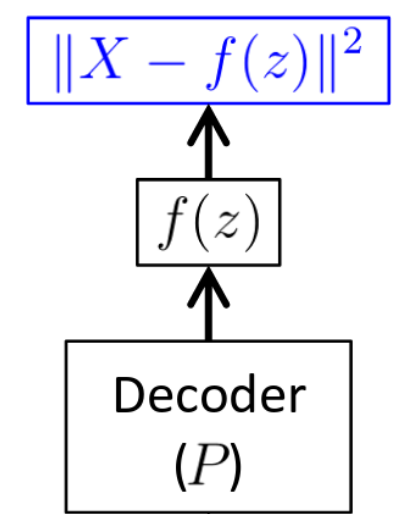
\includegraphics[scale=0.15]{images/vae_decoder.png}};
				\draw[->,thick] (sample.north) -- (decoder.south);
			\end{tikzpicture}
		\end{overlayarea}
		\column{0.6\textwidth}
		\begin{overlayarea}{\textwidth}{\textheight}
			\begin{itemize}\justifying
				\item<1-> Given this setup what should be the loss function for the decoder
				\begin{align*}
					||X - f(z; \theta)||^2
				\end{align*}
				\item<2-> But what about the encoder? What kind of loss function would ensure $\mu$ and $\sigma$ that the encoder produces are the true $\mu$ and $\sigma$ of $P(z|X)$ ?
				\item<3-> Well if we knew the true $P(z)$ then we could have minimized the KL divergence between $Q(z|X)$ and $P(z)$
				\item<4-> But we don't know what $P(z)$ is so we will make an assumption that $P(z)$ is $N(0, I)$
			\end{itemize}
		\end{overlayarea}
	\end{columns}
\end{frame}


\begin{frame}
	\begin{columns}
		\column{0.4\textwidth}
		\begin{overlayarea}{\textwidth}{\textheight}
			% LHS: SHow Figure 2 from tutorial
			\begin{figure}
				\centering
				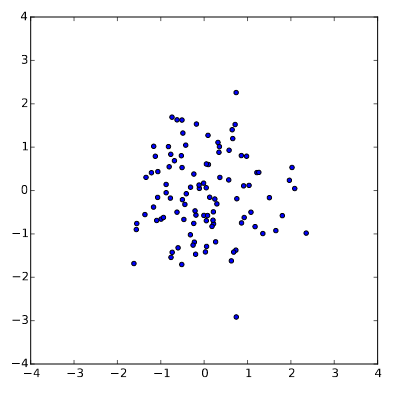
\includegraphics[scale=0.2]{images/2d_dist.png}
			\end{figure}
			\begin{figure}
				\centering
				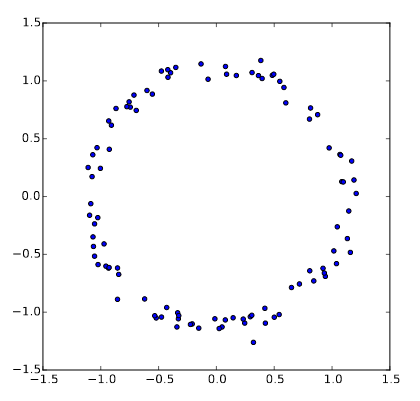
\includegraphics[scale=0.2]{images/2d_trans.png}
			\end{figure}

		\end{overlayarea}
		\column{0.6\textwidth}
		\begin{overlayarea}{\textwidth}{\textheight}
			\begin{itemize}\justifying
				\item<1-> Isn't this is very strong assumption ?
				\item<2-> For example, in the 2-dimensional case how can we be sure that P(z) is a normal distribution and not any other distribution
				\item<3-> The key insight here is that any distribution in d dimensions can be generated by the following steps
				\item<4-> Step 1: Start with a set of d variables that are normally distributed (that's exactly what we are assuming for $P(z)$)
				\item<5-> Step 2: Mapping these variables through a sufficiently complicated function (that's exactly what the first few layers of the decoder can do)
			\end{itemize}
		\end{overlayarea}
	\end{columns}
\end{frame}


\begin{frame}
	\begin{columns}
		\column{0.4\textwidth}
		\begin{overlayarea}{\textwidth}{\textheight}
			% LHS: SHow Figure 2 from tutorial
			\begin{figure}
				\centering
				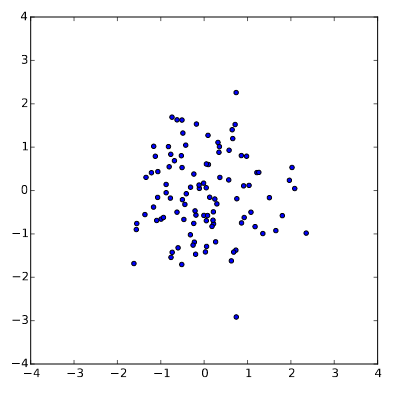
\includegraphics[scale=0.2]{images/2d_dist.png}
			\end{figure}
			\begin{figure}
				\centering
				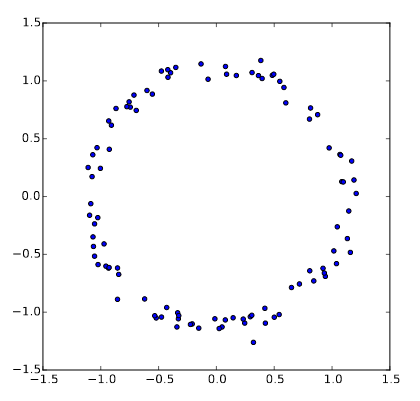
\includegraphics[scale=0.2]{images/2d_trans.png}
			\end{figure}
		\end{overlayarea}
		\column{0.6\textwidth}
		\begin{overlayarea}{\textwidth}{\textheight}
			\footnotesize{\begin{itemize}\justifying
				\item<1-> In particular, note that in the adjoining example if $z$ is 2-D and normally distributed then $g(z)$ is roughly ring shaped (giving us the distribution in the bottom figure)
				\vspace{-4mm}
				\begin{align*}
				g(z) = \frac{z}{10} + \frac{z}{||z||}
				\end{align*}
				\vspace{-6mm}
				\item<2-> In other words, 
				\vspace{-4mm}
				\begin{align*}
				g(z) = \theta_1 z + \theta_2 z
				\end{align*}
				\vspace{-8mm}
				\item<3-> The initial layers of the decoder could learns their weights such that the output is $g(z, \theta)$
				\item<4-> The above argument suggests that even if we start with normally distributed variables the initial layers of the encoder could learn a complex transformation of these variables say $f(z, \theta_1)$ if required
				\item<5-> The objective function of the decoder will ensure that an appropriate transformation of z is learnt to reconstruct $X$
			\end{itemize}}
		\end{overlayarea}
	\end{columns}
\end{frame}


\begin{frame}
	\begin{columns}
		\column{0.4\textwidth}
		\begin{overlayarea}{\textwidth}{\textheight}
			\vspace{4mm}
			\begin{tikzpicture}
				\node[inner sep=0pt] (encoder) at (0,0) {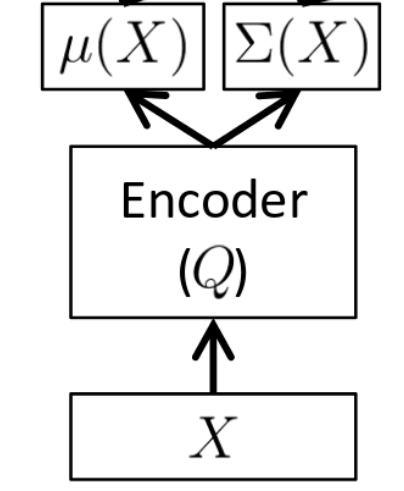
\includegraphics[scale=0.15]{images/vae_encoder.png}};
				\node[inner sep=0pt] (sample) at (0,2) {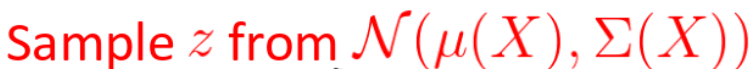
\includegraphics[scale=0.15]{images/vae_sample.png}};
				\draw[->,thick] (encoder.north) -- (sample.south);
				\node[inner sep=0pt] (decoder) at (0,4) {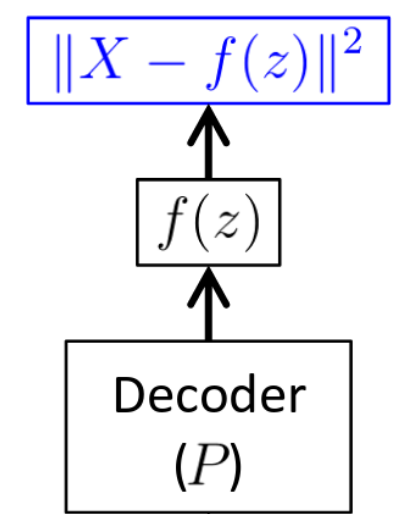
\includegraphics[scale=0.15]{images/vae_decoder.png}};
				\draw[->,thick] (sample.north) -- (decoder.south);
			\end{tikzpicture}
		\end{overlayarea}
		\column{0.6\textwidth}
		\begin{overlayarea}{\textwidth}{\textheight}
			\begin{itemize}\justifying
				\item<1-> So now that we are convinced that it is okay to assume P(z) is N(0, I) then the objective function of the encoder is straightforward
				\item<2-> We simply need to minimize $KL[N(\mu(X), \sigma(X)), N(0, I)]$
				\item<3-> That completes the full picture and we will summarize the discussion on the next slide
			\end{itemize}
		\end{overlayarea}
	\end{columns}
\end{frame}


\begin{frame}
	\begin{columns}
		\column{0.4\textwidth}
		\begin{overlayarea}{\textwidth}{\textheight}
			\vspace{4mm}
			\begin{tikzpicture}
				\node[inner sep=0pt] (encoder) at (0,0) {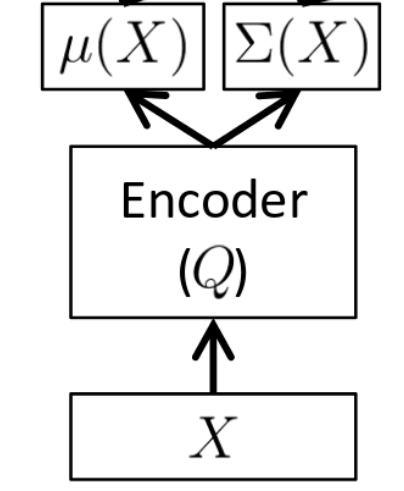
\includegraphics[scale=0.15]{images/vae_encoder.png}};
				\node[inner sep=0pt] (sample) at (0,2) {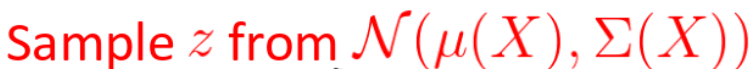
\includegraphics[scale=0.15]{images/vae_sample.png}};
				\draw[->,thick] (encoder.north) -- (sample.south);
				\node[inner sep=0pt] (decoder) at (0,4) {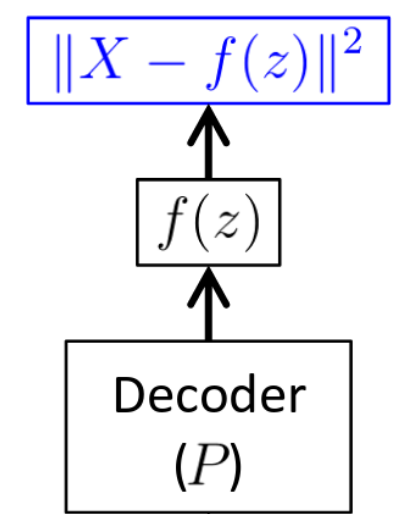
\includegraphics[scale=0.15]{images/vae_decoder.png}};
				\draw[->,thick] (sample.north) -- (decoder.south);
			\end{tikzpicture}
		\end{overlayarea}
		\column{0.6\textwidth}
		\begin{overlayarea}{\textwidth}{\textheight}
			\begin{itemize}\justifying
				\item<1-> Encoder: Generates the $\mu$ and $\sigma$ of $Q(z|X)$
				\item<2-> Decoder: Samples from $Q(z|X)$ and reconstructs $X$
				\item<3-> Encoder loss: 
				\begin{align*}
				min \hspace{3mm}KL[N(\mu(X), \Sigma(X)), N(0, I)]
				\end{align*}
				\item<4-> Decoder loss: 
				\begin{align*}
				min \hspace{3mm}||X - f(z; \theta)||^2
				\end{align*}
				\item<5-> There are still a few pieces missing and we will get back to them later
			\end{itemize}
		\end{overlayarea}
	\end{columns}
\end{frame}


\begin{frame}
	\begin{columns}
		\column{0.4\textwidth}
		\begin{overlayarea}{\textwidth}{\textheight}
			\vspace{4mm}
			\begin{tikzpicture}
				\node[inner sep=0pt] (encoder) at (0,0) {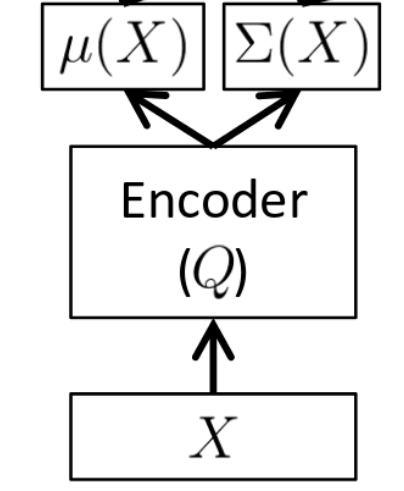
\includegraphics[scale=0.15]{images/vae_encoder.png}};
				\node[inner sep=0pt] (sample) at (0,2) {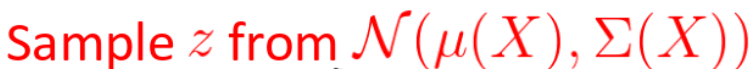
\includegraphics[scale=0.15]{images/vae_sample.png}};
				\draw[->,thick] (encoder.north) -- (sample.south);
				\node[inner sep=0pt] (decoder) at (0,4) {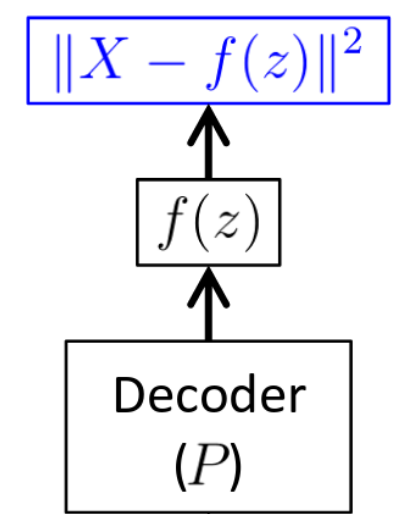
\includegraphics[scale=0.15]{images/vae_decoder.png}};
				\draw[->,thick] (sample.north) -- (decoder.south);
			\end{tikzpicture}
		\end{overlayarea}
		\column{0.6\textwidth}
		\begin{overlayarea}{\textwidth}{\textheight}
			\begin{itemize}\justifying
 				\item<1-> This was a very simplistic (non-rigorous) introduction to VAEs
 				\item<2-> We will now do a more rigorous discussion on the Math behind VAEs
			\end{itemize}
		\end{overlayarea}
	\end{columns}
\end{frame}

